%%%%%%%%%%%%%%%%%%%%%%%%%%%%%%%%%%%%%%
%%%%%%%%%%%%%%%%%%%%%%%%%%%%%%%%%%%%%%
% Do not edit the TeX file your work
% will be overwritten.  Edit the RnW
% file instead.
%%%%%%%%%%%%%%%%%%%%%%%%%%%%%%%%%%%%%%
%%%%%%%%%%%%%%%%%%%%%%%%%%%%%%%%%%%%%%





\newcommand{\DefineMacros}{
\newcommand{\SimNumObs}{5,000}
\newcommand{\SimTrueTheta}{0.5}
\newcommand{\SimAccNumObs}{5,000}
\newcommand{\SimAccSigx}{2}
\newcommand{\SimAccSigeps}{1}
\newcommand{\SimAccPercentMax}{10}

}

%%%%%%%%%%%%%%%%%%%%%%
%%%%%%%%%%%%%%%%%%%%%%
%%%%%%%%%%%%%%%%%%%%%%
% Tables

\newcommand{\CashTransfersResultsTable}{
% \input{figures/cash_transfers_re_run_table.tex}


\begin{table}\tiny 
\begin{tabular}{|ccccc|}
\toprule
Study case & Original estimate  & Target change  & Refit estimate  & Observations dropped \\
\midrule
\midrule
& &  Sign change &  \textbf{-2.559 (3.541)} &  697 = 6.63\%\\
Poor, period 10  &  33.861 (4.468)* &  Significance change &  \textbf{4.806 (3.684)} &  435 = 4.14\%\\
& &  Significant sign change &  \textbf{-9.416 (3.296)*} &  986 = 9.37\%\\
\midrule
& &  Sign change &  \textbf{-0.573 (6.750)} &  30 = 0.70\%\\
Non-poor, period 10  &  21.493 (9.405)* &  Significance change &  \textbf{16.262 (8.927)} &  3 = 0.07\%\\
& &  Significant sign change &  -10.845 (6.467) &  92 = 2.16\%\\
\midrule
\bottomrule
\end{tabular}
\caption{ Cash transfers results for the final study period. The ``Refit estimate'' column shows the result of re-fitting the model removing the Approximate Most Influential Set. Stars indicate significance at the 5\% level.  Refits that achieved the desired change are bolded. }
\label{table:cash_transfers_re_run_table}
\end{table}


}

%%%%%%%%%%%%%%%%%%%
% OHIE

% \newcommand{\OHIEResultsTable}{
% % \input{figures/OHIE_table_9_IV_re_run_table.tex}
% <<OHIE_results_table, cache=ohie_cache, results='asis'>>=
% source("figures_knitr/OHIE/OHIE-table_results.R",
%        echo=knitr_debug, print.eval=TRUE)
% @
% }


%%%%%%%%%%%%%%%%%%%
% Microcredit
%
% \newcommand{\MicrocreditProfitResultsTable}{
% % \input{figures/microcredit_profit_re_run_table.tex}
% <<microcredit_profit_results_table, cache=microcredit_cache, results='asis'>>=
% source("figures_knitr/microcredit/microcredit_profit_results_table.R",
%        echo=knitr_debug, print.eval=TRUE)
% @
% }
%
%
% \newcommand{\MicrocreditTemptationResultsTable}{
% % \input{figures/microcredit_profit_re_run_table.tex}
% <<microcredit_temptation_results_table, cache=microcredit_cache, results='asis'>>=
% source("figures_knitr/microcredit/microcredit_temptation_results_table.R",
%        echo=knitr_debug, print.eval=TRUE)
% @
% }

%%%%%%%%%%%%%%%%%%%
% Microcredit mixture
%
% \newcommand{\MicrocreditMixtureResultsTable}{
% <<mcmix_re_run_table, cache=mcmix_cache, results='asis'>>=
% source("figures_knitr/microcredit_mixture/microcredit_mix_refit_table.R",
%        echo=knitr_debug, print.eval=TRUE)
% @
% }
%
% \newcommand{\MicrocreditMixtureSdResultsTable}{
% <<mcmix_sd_re_run_table, cache=mcmix_cache, results='asis'>>=
% source("figures_knitr/microcredit_mixture/microcredit_mix_sd_refit_table.R",
%        echo=knitr_debug, print.eval=TRUE)
% @
% }

%%%%%%%%%%%%%%%%%%%%%%
%%%%%%%%%%%%%%%%%%%%%%
%%%%%%%%%%%%%%%%%%%%%%
% Graphs


\newcommand{\SimApproxNormalGraph}{

\begin{knitrout}
\definecolor{shadecolor}{rgb}{0.969, 0.969, 0.969}\color{fgcolor}\begin{figure}[!h]

{\centering 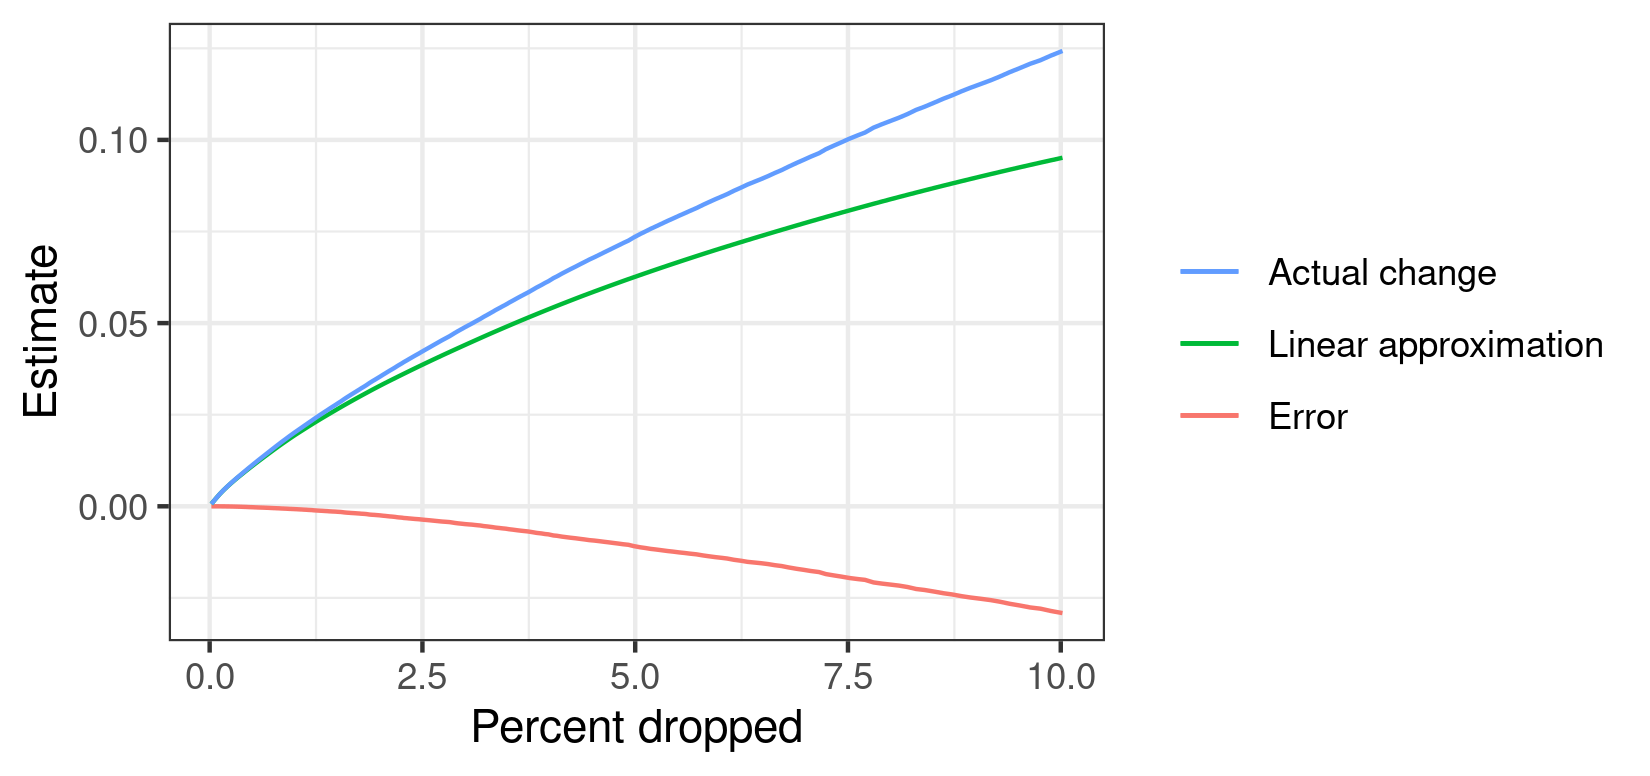
\includegraphics[width=0.98\linewidth,height=0.461\linewidth]{figure/sim-approx-normal-1} 

}

\caption[The actual change, linear approximation to the change, and approximation error.Here, $\sigma_x = \SimAccSigx$, $\sigma_\varepsilon = \SimAccSigeps$, and $\theta_0 = \SimTrueTheta$]{The actual change, linear approximation to the change, and approximation error.Here, $\sigma_x = \SimAccSigx$, $\sigma_\varepsilon = \SimAccSigeps$, and $\theta_0 = \SimTrueTheta$.}\label{fig:sim-approx-normal}
\end{figure}


\end{knitrout}
}

\newcommand{\SimGridNormalGraph}{

\begin{knitrout}
\definecolor{shadecolor}{rgb}{0.969, 0.969, 0.969}\color{fgcolor}\begin{figure}[!h]

{\centering 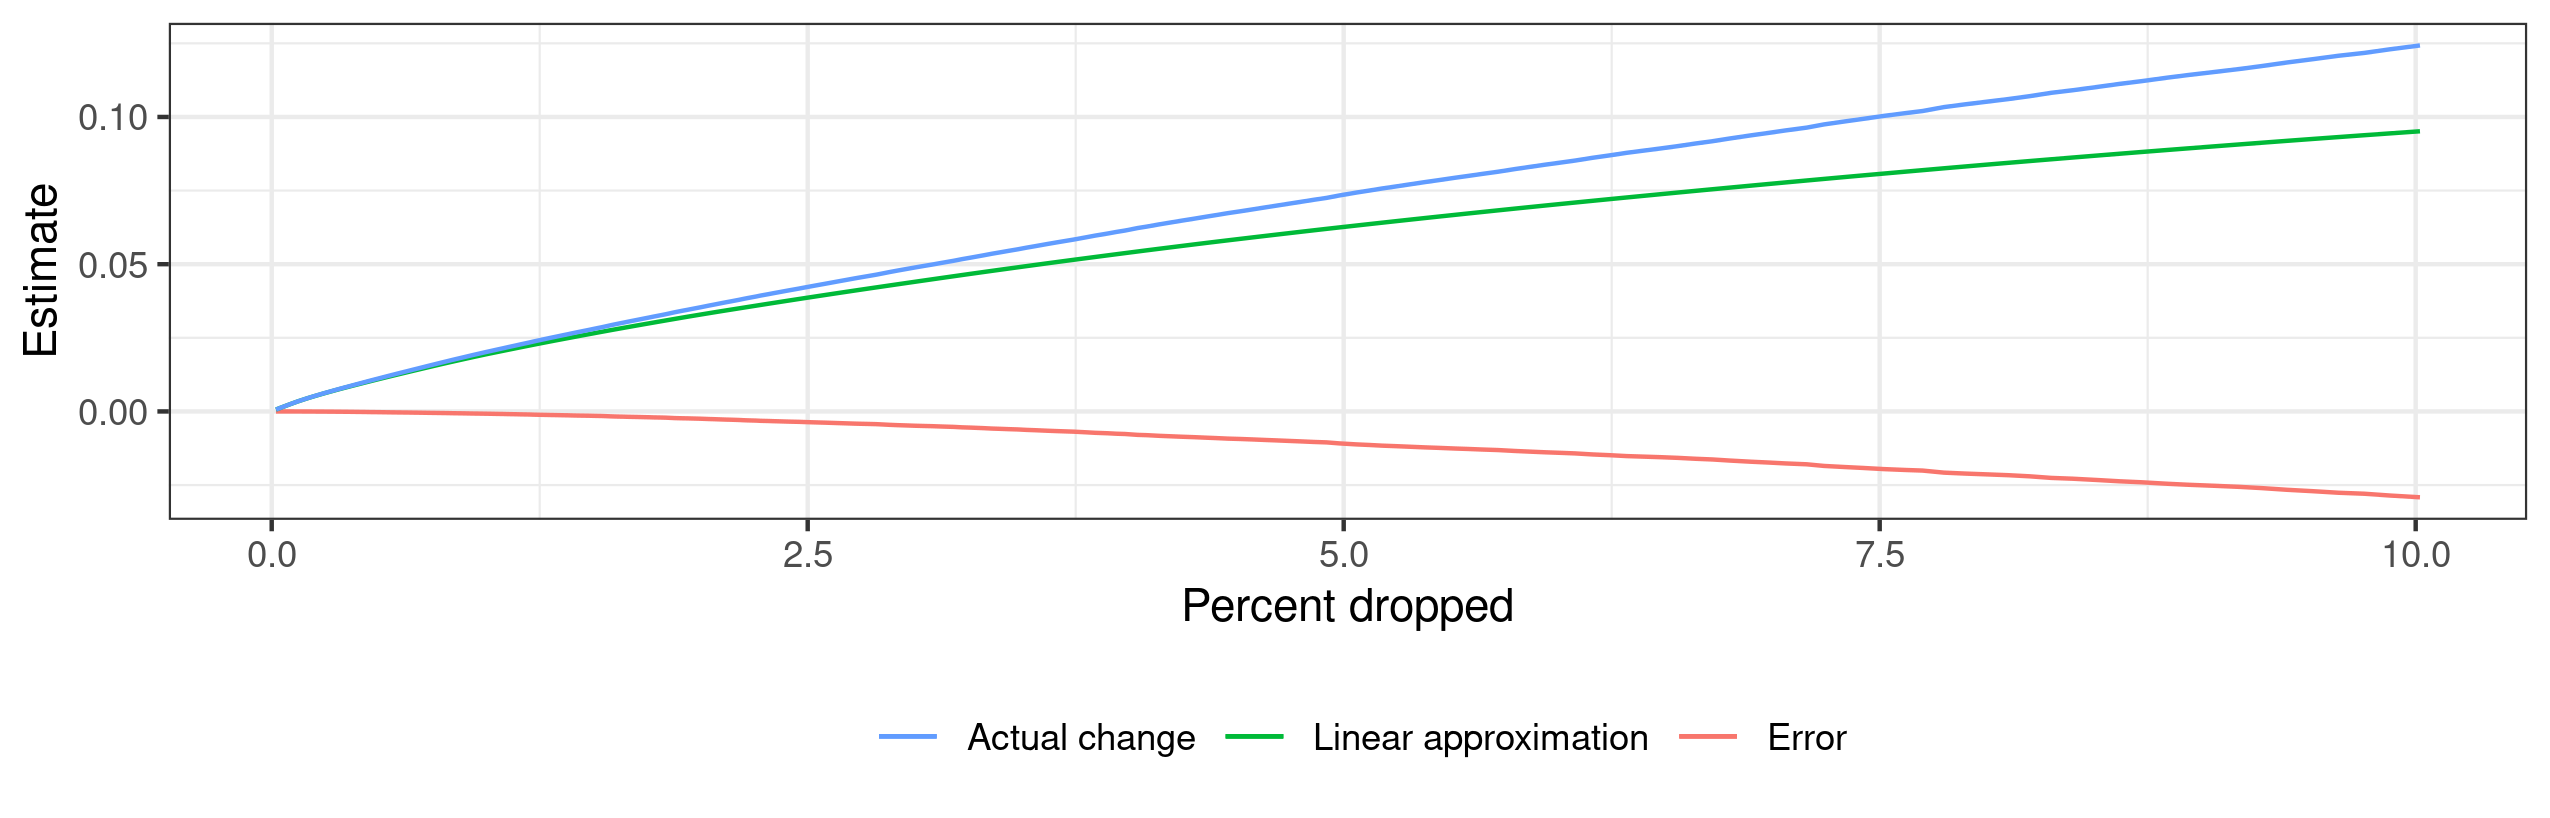
\includegraphics[width=0.98\linewidth,height=0.384\linewidth]{figure/sim-grid-normal-1} 

}

\caption[The approximate perturbation inducing proportion at differing values of $\sigma_x$ and $\sigma_\varepsilon$]{The approximate perturbation inducing proportion at differing values of $\sigma_x$ and $\sigma_\varepsilon$. Red colors indicate datasets whose sign can is predicted to change when dropping less than 1\% of datapoints. The grey areas indicate $\amip{\alpha} = \na$, a failure of the linear approximation to locate any way to change the sign.}\label{fig:sim-grid-normal}
\end{figure}


\end{knitrout}
}
